\documentclass[a4paper]{article}

\usepackage[utf8]{inputenc}
\usepackage{minted}
\usepackage{listings}
\usepackage{amssymb, amsfonts, latexsym, amsthm, amsmath, framed}
\usepackage{esvect}
\usepackage{parskip}

\usepackage{amsmath, amssymb, framed, tcolorbox}
\tcbuselibrary{theorems}

\usepackage{graphicx}

\usepackage{mathrsfs}

\usepackage{xcolor}

\usepackage[demo]{graphicx}
\usepackage{babel,blindtext}

\usepackage[colorlinks,linkcolor=blue,citecolor=blue,urlcolor=blue]{hyperref} % 

%% Bibliography support
\usepackage[backend=bibtex,isbn=false,url=false]{biblatex} 

\addbibresource{ref.bib}

\newcommand{\ba}{\backslash}
\newcommand{\Q}{\mathbb{Q}}
\newcommand{\C}{\mathbb{C}}
\newcommand{\R}{\mathbb{R}}
\newcommand{\N}{\mathbb{N}}
\newcommand{\Z}{\mathbb{Z}}
\newcommand{\F}{\mathbb{F}}
\newcommand{\rank}{\text{rank}}



% figure support
\usepackage{import}
\usepackage{xifthen}
\pdfminorversion=7
\usepackage{pdfpages}
\usepackage{transparent}
\newcommand{\incfig}[1]{%
	\def\svgwidth{\columnwidth}
	\import{./figures/}{#1.pdf_tex}
}

\newtheoremstyle{bfnote}%
  {}{}
  {}{}
  {\bfseries}{.}
  { }{\thmname{#1}\thmnumber{ #2}\thmnote{ (#3)}}

\theoremstyle{bfnote} % set the style for the following theorems

\newtheorem{thm}{Theorem}[section] %\newtheorem{name}{display-text}[numbered-within]

\newtheorem{lem}[thm]{Lemma} %\newtheorem{name}[numbered-like]{display-text}
\newtheorem{cor}[thm]{Corollary}
\newtheorem{prop}[thm]{Proposition}
\newtheorem{alg}[thm]{Algorithm}

\theoremstyle{bfnote}                  % switch to a different style
\newtheorem{defn}[thm]{Definition}
\newtheorem{conj}[thm]{Conjecture}


\theoremstyle{example}                       % another style
\newtheorem{prob}[thm]{Problem}


\theoremstyle{remark}                       % another style
\newtheorem{exmp}[thm]{Example}  % (note:the "example" style is not really good for long examples-- typesets them in italics!)
\newtheorem{rem}[thm]{Remark}
\newtheorem{claim}[thm]{Claim}
\renewcommand{\theclaim}{}

%% If you use numbered equations in a long document, it is preferred to number
% as (x.y), where x is section number, y is equation number

\numberwithin{equation}{section}

\pdfsuppresswarningpagegroup=1

\title{Theorem Prover on Analysis Topics}
\date{Spring 2022, Analysis 2}
\author{Yuxuan Sun}

\begin{document}

\maketitle
\tableofcontents

\section{Introduction}
Mathematical proofs could get more difficult to read and verify as they grow to be more complicated. What else could we rely on to verify the proofs are correct besides trust on each other's professionalism? Building on homotopy type theory, automated theorem proving has the ability to verify our proofs. As there are many modern theorem provers, such as Agda, Lean, Coq, the intention of the paper is to give a brief introduction on how to construct basic analysis definitions and to prove theorems using \textit{Lean}, with sufficient explanations for mathematicians on how the language works.

When preparing for this paper, I mainly rely on \cite{Avigad2016} and \cite{homotopy}. The choice of using \textit{Lean} is based on \cite{boldo}. Since the paper in general comes from understanding the mixture of the sources and the online library of \textit{Lean}, I won't be able to cite them separately in below.

We will start with some very mathematically simple definitions and proofs, then move to a sequence-limit proof in Analysis I. Due to page limit, I will briefly introduce what the proofs related to functional analysis look like at the end.

\section{Basic Definition and Proofs}

Specifically, let's look at the definition of upper bounds written in Lean.

\begin{listing}[!ht]
\begin{minted}[escapeinside=||,mathescape=true]{c}
def upperBounds (A : set |$\R$|) := { x : |$\R \quad \vert \quad  \forall $| a |$\in $| A,  a |$\le$| x }
\end{minted}
\end{listing}

Here we defined a function named \texttt{upperBounds}, which takes one input: \texttt{A} whose \textbf{type} is a set of real numbers. The output of the function is a set (indicated by $\left\{ \quad \right\} $, and the type of elements \texttt{x} in the set is real numbers.  \texttt{x}  also need to satisfy the property that for all \texttt{a} $\in $ \texttt{A}, \texttt{a} $\le $ \texttt{x}.

We could also define the maximum element in a set as the following.

\begin{listing}[!ht]
\begin{minted}[escapeinside=||,mathescape=true]{c}
def isMaximum (a : |$\R$|) (A : set |$\R$|) := a |$\in$| A |$\land$| a |$\in$| upperBounds A
\end{minted}
\end{listing}

This function \textbf{isMaximum} takes two inputs: \texttt{a} whose type is real number; \texttt{A} whose type is a set of real numbers.

Its output is a boolean: \texttt{a} is in \texttt{A}  \textbf{and} \texttt{a} is in upperBounds \texttt{A}. Notice that here we called the function we defined above so upperBounds A is the output of the function defined above.

An observation is that since the logical connection here is \textbf{and}, if \textbf{isMaximum a A} returns true, we are guaranteed two truth statements: $a$ is in  $A$ and  $a$ is in upperBounds A.  

\bigskip

Now we could prove something! 

Let's prove that if both  $x$ and  $y$ are maximum of  $A$, then  $x = y$

\subsection{details of the first proof}
First a longer and more detailed proof is the following.

\begin{minted}[xleftmargin=20pt,linenos,escapeinside=||, mathescape=true]{c}
lemma uniqueMax (A : set |$\R$|) (x y : |$\R$|) 
(hx : isMaximum x A) (hy : isMaximum y A) 
: x = y 
:= 
begin
	cases hx with x_in x_up,
	cases hy with y_in y_up,
	specialize x_up y,
	specialize x_up y_in,
	specialize y_up x x_in,
	linarith,
end

\end{minted}	


The lemma takes four assumptions: 

\textbf{1. }\texttt{A} whose type is a set of real numbers

\textbf{2. }\texttt{x,y} whose types are real numbers

\textbf{3. }\texttt{hx} whose type is a boolean derived from \texttt{isMaximum} above. Recall that then it contains two statements: 

\quad\textbf{a.} x is in A

\quad\textbf{b.} x is in upperBounds A (x is bigger than anything in A)

\textbf{4. }\texttt{hy} is similar as \texttt{hx} 

Assumptions are usually stated before colon \textbf{:}

After the colon it's the result we want to prove, namely: $x = y$

\textbf{:=} indicates that  our proof begins.

Now let's look at the details of the proof.

At line 6, we have \texttt{cases ... with ...}, operations like this are called tactics in \textit{Lean}. It splits the hypothesis \texttt{hx} into two pieces, named \texttt{x\_in} and \texttt{x\_up}, corresponding to \textbf{3a} and \textbf{3b} respectively, because \texttt{hx} is a conjunction, it will be easier for us to use.

Similarly for line 7.

At line 8, \texttt{specialize} is a tactic which applies everything following the first thing to the first thing. In this line, it gives the hypothesis \texttt{x\_up} the number \texttt{y}, so now our \texttt{x\_up} is renewed as: \texttt{y $\in$ A $\to$ y $\le$ x}

At line 9, in order to have \texttt{y} $\le$ \texttt{x}, we need to give our new \texttt{x\_up} the precedent: \texttt{y} is in \texttt{A}, which is provided by  \texttt{y\_in}. After line 9, our proof so far has shown that $y \le x$.

At line 10, it's just a quicker way to write line 8 and 9 together.

\texttt{linarith} is a basic linear arithmetic package lean has that allow us to turn $ x \le y$ and $y \le x$ into $x =y$. Thus our proof is done.

One feature \textit{Lean} has is that as you are writing proofs, it could tell you how your hypothesis has been updated, as shown below.

\begin{figure}[!htb]
\minipage{0.32\textwidth}
  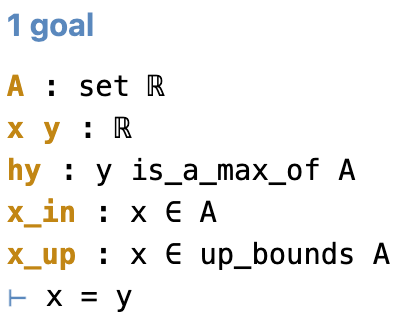
\includegraphics[width=\linewidth]{line6.png}
  \caption{At line 6}\label{fig:awesome_image1}
\endminipage\hfill
\minipage{0.32\textwidth}
  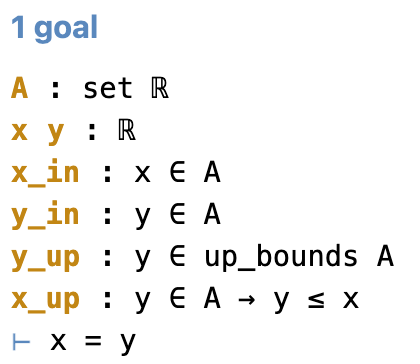
\includegraphics[width=\linewidth]{line8.png}
  \caption{At line 8}\label{fig:awesome_image2}
\endminipage\hfill
\minipage{0.32\textwidth}%
  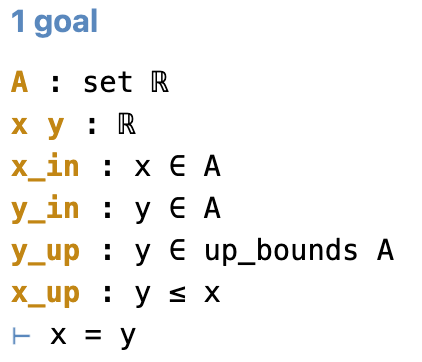
\includegraphics[width=\linewidth]{line9.png}
  \caption{At line 9}\label{fig:awesome_image3}
\endminipage
\end{figure}

\subsection{simplified first proof}
Certainly, for a simple proof, we could also write a shorter version (next page).

\begin{listing}[!ht]
\begin{minted}[xleftmargin=20pt,linenos,escapeinside=||, mathescape=true]{c}
lemma uniqueMax (A : set |$\R$|) (x y : |$\R$|) 
(hx : isMaximum x A) (hy : isMaximum y A) 
: x = y 
:= 
begin
	have : x |$\le $| y, from hy.2 x hx.1,
	have : y |$\le$| x, from hx.2 y hy.1,
	linarith,
end
\end{minted}
	
\end{listing}

\texttt{have from} is a tactic which produce a hypothesis by applying what's following from. Here  \texttt{hy.2} refers to the second part of  \texttt{hy}, which is \texttt{y $\in$ upperBounds A}.

The advantages of writing proofs in this way is straightforward: it's shorter. However, it does decrease the readability of the proof, as it's hard for readers to know what  \texttt{hy.2} refers to. 



\section{Sequence-Limit Definition and Proof}

Let's prove another thing in analysis, namely, given two sequences $u_n, v_n$, if $u_n \to l$ and $v_n \to l'$ then $(u_n + v_n) \to (l+l')$

Before that, we need the definition of sequence-limit.

\begin{minted}[xleftmargin=20pt,linenos,escapeinside=||, mathescape=true]{c}
def seq_limit (u : |$\N \to \R$|) (l : |$\R$|) : Prop :=
|$\forall \epsilon > 0, \exists $| N, |$\forall$| n |$\ge$| N, |$\mid$|u n - l|$\mid$| |$\le  \epsilon$|
\end{minted}	

Let's go straight to the proof and explain the details later.

\begin{listing}[!h]
\begin{minted}[xleftmargin=20pt, linenos,escapeinside=||, mathescape=true]{c}
lemma sequenceAdd (hu : seq_limit u l1) (hv : seq_limit v l2) :
seq_limit ( u + v) (l1 + l2)
:=
begin
	intros |$\epsilon$| |$\epsilon$|_pos,
	cases hu (|$\epsilon$|/2) (by linarith) with N1 hN1,
	cases hv (|$\epsilon$|/2) (by linarith) with N2 hN2,
	use max N1, N2,
	intros n hn,
	rewrite ge_max_iff at hn,
	calc
	|$\mid$| (u + v) n - (l1 + l2) |$\mid$| = |$\mid$| un + vn - (l1 + l2) |$\mid$| :rfl 
	. . . = |$\mid$| (u n - l1) + (v n - l2) |$\mid$| : by congr 1; ring 
	. . . |$\le$| |$\mid$| un - l1 |$\mid$| + |$\mid$| vn - l2 |$\mid$| : by apply abs_add 
	. . . |$\le$| |$\epsilon$| : by linarith [hN1 n (by linarith), hN2 n (by linarith)]
end
\end{minted}
\end{listing}
The places with \texttt{intros} and \texttt{cases} are similar as our basic example. It a more complicated usage but the ideas are similar: \texttt{intros} give names to what we had and \texttt{cases} splits the hypothesis so that we could use them later.

In line 7, we use a library function named \texttt{max} to take the maximum of \texttt{N1, N2}. Later in line 8, we use \texttt{n} to denote the number and \texttt{hn} to denote the statement that \texttt{n} $\ge$ \texttt{max N1 N2}.

In line 8, we rewrite \texttt{hn} using a library function named  \texttt{ge\_max\_iff}, which just split \texttt{hn} into \texttt{n} $\ge$ \texttt{N1} $\wedge$  \texttt{n} $\ge $ \texttt{N2}. 

In line 8, since it's just splitting and renaming, we could also write \[
	\texttt{cases ge\_max\_iff.mp hn with hn1 hn2}
\] 
Starting at line 11, one could just consider it as an align environment in latex with reasons mandatorily required. Whatever is following \texttt{by} are library theorems, whose meanings one could probably guess.

Notice that at line 15, the square bracket after linarith is a quicker way to write the following.
\begin{minted}[xleftmargin=20pt, linenos,escapeinside=||, mathescape=true]{c}
have fact1 :  |$\mid$|u n - l1|$\mid$| |$\le$| |$\epsilon$|/2,
    from hN1 n (by linarith),
have fact2 : |$\mid$|v n - l2|$\mid$| |$\le$| |$\epsilon$|/2,
    from hN2 n (by linarith),
\end{minted}

For reference, before line 11, what we built up is shown in Figure \ref{sequence}.

\begin{figure}[h!]
 \centering
 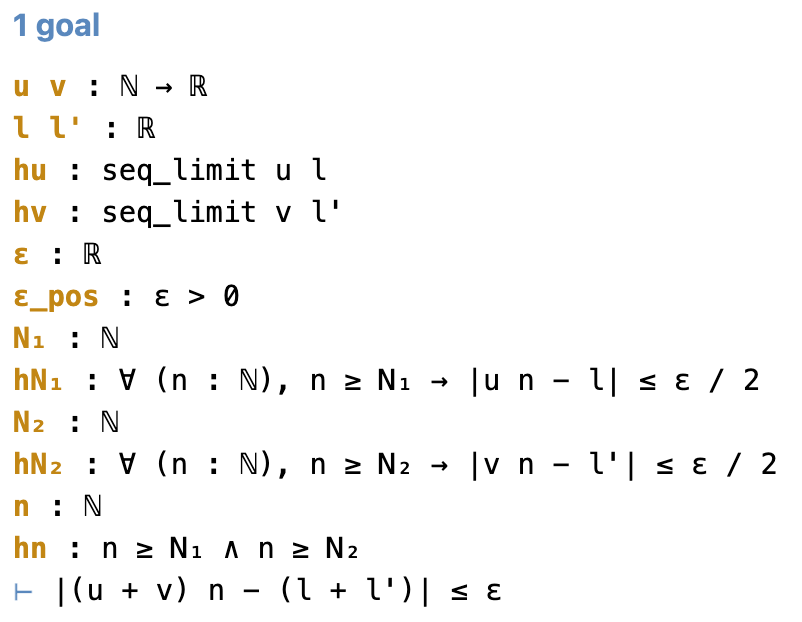
\includegraphics[width=3 in]{sequence}
 \caption{Before line 11 (cursor at line 10)}
 \label{sequence}
 \end{figure}
\section{Functional Analysis}
Recall what we learnt in class about functions in $L^1$.
\begin{thm}[$L^1(\R)$ closed under addition]
	Given $f_1, f_2 \in L^1(\R)$, then $f_1+f_2 \in L^1(\R)$, namely \[
		\int_{-\infty}^{\infty} f_1(x) + f_2(x) dx = \int_{-\infty}^{\infty} f_1(x) dx + \int_{-\infty}^{\infty} f_2(x) dx
	\] 
\end{thm}
The statement of it is the following.
\begin{listing}[!ht]
\begin{minted}[escapeinside=||, mathescape=true]{c}
lemma lintegral_nnnorm_add
  {f : a |$\to$| b} {g : a |$\to$| y} 
  (hf : ae_strongly_measurable f u) 
  (hg : ae_strongly_measurable g u) 
  : |$ \int^- $| a, nnnorm (f a) + nnnorm (g a) du = 
  	|$\int^-$| a, nnnorm (f a) du + |$\int^-$| a, nnnorm (g a) du	
\end{minted}
\end{listing}
\texttt{nnnorm} here is the notation we use when talk about functions.

Due to the page limit and the length of the proof (it could be really short by using a bunch of library functions but really long if we spell everything out). The proof is omitted. It is long mainly because that we need to seriously take about measures.

The takeaway here may be my failed attempt of writing it in the ``hand-wavy'' way we did in class, where we skipped the detailed discussions on measure. I have not figured out a way to do so such that the prover would accept.

\section{Discussion}
The power of using theorem prover is obvious: it's an insurance of our mathematical correctness. However as I go along the process my major thought is: is it worth it?

Using theorem prover, especially one with sufficient libraries to use, shares the deficit of all other programming languages, it could be hard to read sometimes if the code is abbreviated. However, advanced mathematical proofs also have this problem, as sometimes it could even be hard to understand when the content is the same but notations are different. In theorem prover, at least one could keep tracing back until one finds the source code that the writer is using.

In conclusion, I hope this paper gives a comprehensive introduction on theorem prover to mathematicians who are not familiar with programming languages at all, and maybe some motivations to try to use it in some of their works.

\newpage
\printbibliography
\end{document}












